
\section{Weiterführende Konzeption: Vom IFC-Modell zur Robotermission}\label{sec:Weiterführung}
\subsection{Verarbeitungskette und roboterspezifisches Exportformat}

Ausgangspunkt der weiterführenden Robotikverarbeitung ist die annotierte IFC-Datei. Im aktuellen
Editorstand werden Robotermissionen und ihre Aufgaben mit konkreten IFC-Gebäudeelementen verknüpft
und in die IFC-Datei überführt. Ebenso ist der umgekehrte Weg umgesetzt: Vom System erzeugte
Missionsannotationen können aus einer direkt geladenen IFC-Datei rekonstruiert, im Editor bearbeitet
und erneut exportiert werden. Die annotierte IFC-Datei bildet damit den fachlichen und
gebäudebezogenen Ausgangsträger der Mission. Die Aktionssemantik liegt auf Task-Ebene; das
referenzierte Gebäudeelement bleibt davon als eigenständig identifizierbares IFC-Objekt getrennt.

Die gewählte IFC-Abbildung enthält bereits einen wesentlichen Teil der für die Missionsbeschreibung
erforderlichen Informationen. Eine Mission wird durch Aufgaben konkretisiert, zwischen denen eine
Ausführungsreihenfolge definiert werden kann. Die Aufgaben tragen die projektspezifische
Aktionssemantik und verweisen auf die Gebäudeelemente, auf die sich die jeweilige Aktion bezieht.
IFC stellt hierfür allgemeine Prozess-, Beziehungs- und Identitätsmechanismen bereit.
\textit{IfcTask} kann eine identifizierbare Arbeitseinheit repräsentieren, \textit{IfcRelSequence}
zeitliche beziehungsweise logische Abhängigkeiten zwischen Prozessen ausdrücken und
\textit{IfcRelAssignsToProcess} Prozesse mit denjenigen Objekten verknüpfen, auf denen sie
operieren. Von \textit{IfcRoot} abgeleitete Objekte verfügen zudem über einen \textit{GlobalId}, der
als stabiler Identifikationsanker für den Objektbezug genutzt werden kann. Die normative Bedeutung
dieser Entitäten sollte in der endgültigen Textfassung über die buildingSMART-IFC-Spezifikation
belegt werden.

Damit enthält die annotierte IFC-Datei nicht nur geometrische Zielobjekte, sondern die fachliche
Verbindung zwischen Gebäude und Mission.Eine Aufgabe kann beispielsweise ausdrücken, dass eine
bestimmte Tür geöffnet, durchquert und anschließend wieder geschlossen werden soll. Die
referenzierte Tür bleibt dabei dasselbe Gebäudeelement mit eigener IFC-Identität; die
unterschiedlichen Aktionen gehören zu den jeweiligen RobotTasks. Dasselbe Bauteil kann folglich in
mehreren aufeinanderfolgenden Tasks mit unterschiedlicher Bedeutung vorkommen. Die Missionssemantik
wird damit nicht in das Gebäudeelement selbst verlagert, sondern über die Annotation mit diesem
verknüpft.

Für nachgelagerte Robotikkomponenten ist es dennoch nicht zweckmäßig, in jedem Verarbeitungsschritt
unmittelbar mit der vollständigen IFC-Struktur zu arbeiten. Ein IFC-Modell enthält neben der Mission
unter anderem räumliche Hierarchien, Bauteilgeometrien, Materialien, Eigenschaftssätze und
zahlreiche Beziehungen, von denen eine Navigations- oder Ausführungskomponente nur einen Ausschnitt
benötigt. Eine roboterspezifische Austauschrepräsentation kann diesen Ausschnitt explizit
strukturieren und um Informationen ergänzen, die erst bei der Überführung in die Robotikdomäne
entstehen. Der Nutzen einer solchen Transformation wird auch in verwandten Arbeiten sichtbar. Gopee,
Prieto und García de Soto (2023) leiten aus IFC unter anderem 2D-Hinderniskarten, semantische
JSON-Daten und Wegpunkte für autonome Robotersysteme ab. Zhu, Pauwels und De Vries (2023) verfolgen
für einen anderen Anwendungsfall eine automatisierte Transformation von IFC in das Simulation
Description Format, um BIM-Informationen in einer ROS-/Gazebo-basierten Simulationsumgebung nutzbar
zu machen. Beide Arbeiten verwenden nicht das hier entwickelte Missionsannotationsmodell, zeigen
aber denselben grundlegenden Bedarf, umfassende BIM-Daten in eine für konkrete Robotikkomponenten
zweckgebundene Repräsentation zu überführen.

Diese zusätzliche Repräsentation ist nicht als zweite kanonische Projektdatei zu verstehen. Die
fachliche Mission verbleibt in der annotierten IFC-Datei. Ein roboterspezifischer Export ist
vielmehr ein daraus abgeleitetes und grundsätzlich erneut erzeugbares Ausführungsartefakt.
Änderungen an Aufgaben, Reihenfolge oder IFC-Objektbezügen werden weiterhin in der fachlichen
Ausgangsrepräsentation vorgenommen; die roboterspezifische Repräsentation kann anschließend neu
erzeugt werden. Dadurch wird vermieden, zwei voneinander unabhängige Missionsbeschreibungen
dauerhaft synchron halten zu müssen.

Eine experimentelle Ausprägung dieser Schnittstelle wurde in einem separaten Backend-orientierten
Versuchsaufbau untersucht. Dieser ist nicht Bestandteil des browserbasierten Editors. Dort wird die
annotierte IFC-Datei mit IfcOpenShell eingelesen; Mission, Task-Reihenfolge und referenzierte
Gebäudeelemente werden rekonstruiert und um abgeleitete räumliche Informationen ergänzt. Die
erzeugte JSON-Repräsentation enthält unter anderem Missionsidentifikation, geordnete Tasks,
Aktionssemantik, IFC-Objektreferenzen und Angaben zum räumlichen Bezugssystem. Zusätzlich können
Wegpunkte, deren Zuordnung zu Aktionen und Pfadsegmente zwischen aufeinanderfolgenden Wegpunkten
ausgegeben werden.

Die in Kapitel 6 verwendete Kette

**annotierte IFC-Datei → RobotTasks → roboterspezifische Austauschrepräsentation → Navigationsziele → Navigationsdarstellung → Pfad**

ist dabei als fachliche Transformationsfolge zu verstehen. Sie beschreibt die zunehmende
Spezialisierung der Informationen in Richtung Robotik. Daraus folgt nicht, dass jeder Schritt
technisch zwingend eine Datei schreiben muss, die vom nächsten Schritt wieder eingelesen wird. Im
experimentellen Versuchsaufbau können mehrere Artefakte aus demselben rekonstruierten Missions- und
Gebäudekontext abgeleitet werden. Insbesondere ist das \textit{robot.json} eine konkrete
Serialisierung der roboterspezifischen Sicht, nicht notwendigerweise der technische Eingabekanal für
jeden nachfolgenden Verarbeitungsschritt.

Für die Datenmodellierung ist die Trennung zwischen RobotTask und Waypoint zentral. Ein RobotTask
beschreibt fachlich, was innerhalb der Mission geschehen soll. Ein Waypoint beschreibt räumlich,
an welchem Navigationspunkt ein Bewegungs- oder Interaktionsschritt stattfinden soll. Zwischen
beiden besteht deshalb keine zwingende Eins-zu-eins-Beziehung. 

\begin{figure}[htbp]
  \centering
  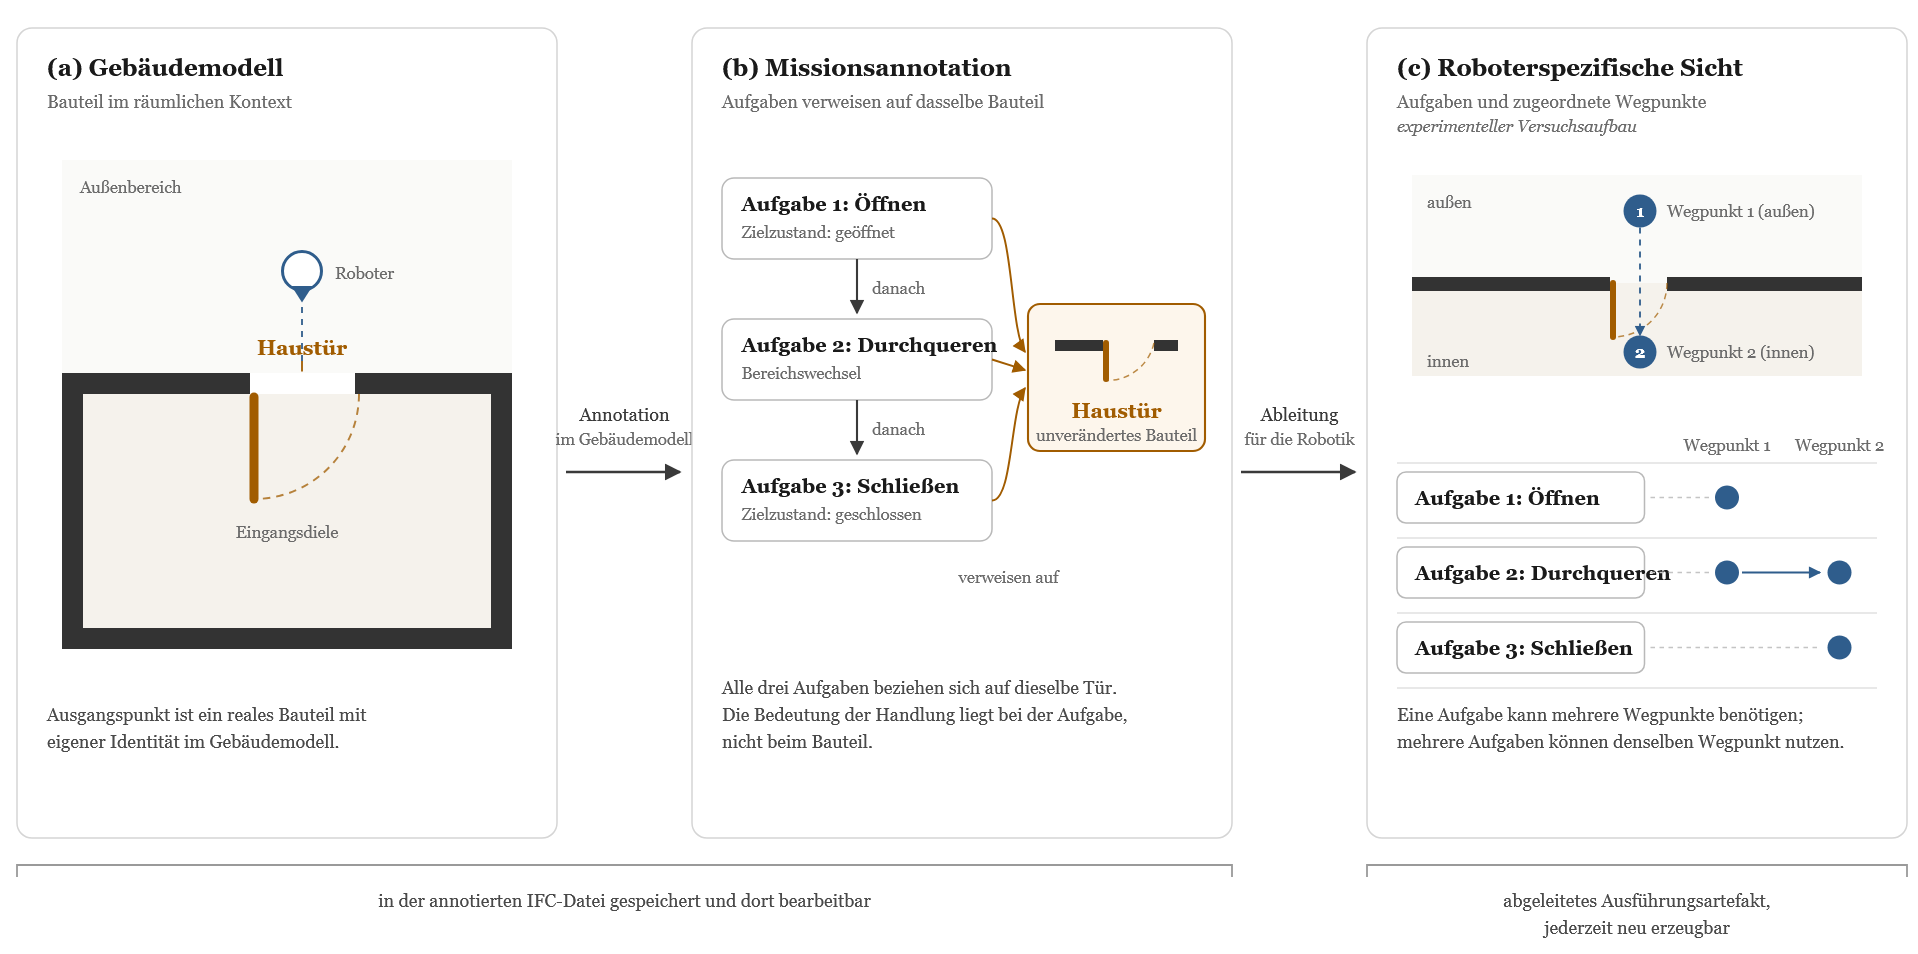
\includegraphics[width=\textwidth]{pics/Gebaeudebezug.png}
  \caption{Vom Gebäudeelement zur roboterspezifischen Missionsrepräsentation.}
  \label{fig:gebaeudebezug-mission}
\end{figure}

Beim Öffnen und anschließenden Durchqueren einer Tür können beispielsweise mehrere Aktionen denselben Punkt auf einer Türseite
verwenden, während eine einzelne Aktion wie \textit{PASS\_THROUGH} eine Eintritts- und eine
Austrittsseite und damit mehrere Wegpunkte benötigt. Die genaue geometrische Ableitung dieser Punkte
wird in Abschnitt 6.2 behandelt.

Diese Trennung ist für die Erweiterbarkeit wesentlich. Würde jede fachliche Aufgabe unmittelbar auf
genau eine Position reduziert, gingen Informationen über Aktionen verloren, die mehrere räumliche
Zustände benötigen. Umgekehrt würden mehrere unmittelbar aufeinanderfolgende Aktionen am gleichen
Ort unnötigerweise zu mehreren identischen Navigationsstopps führen. Die explizite Relation zwischen
Tasks und Wegpunkten erlaubt dagegen, semantische Missionsstruktur und räumliche Navigation
unabhängig voneinander weiterzuentwickeln. Ein anderer Robotertyp oder eine geänderte Methode zur
Zielableitung kann zu anderen Anfahrpunkten führen, ohne dass hierfür die ursprüngliche
Task-Semantik im IFC-Modell verändert werden muss.

Für die Austauschrepräsentation ist außerdem zwischen fachlich dauerhaften, abgeleiteten und
laufzeitabhängigen Informationen zu unterscheiden. Dauerhaft sinnvoll sind insbesondere die
Identifikation und Version des Exportformats, die geordnete Task-Struktur, Aktionssemantik und
Aktionsparameter sowie stabile Referenzen auf die betroffenen IFC-Objekte. Räumliche Daten benötigen
zusätzlich eine eindeutige Beschreibung von Einheit und Koordinatenrahmen. Bereits vor der
Ausführung berechnete Anfahrpunkte, Wegpunkte oder Pfade können ebenfalls exportiert werden, sind
jedoch abgeleitete Informationen. Ihre Gültigkeit hängt unter anderem vom zugrunde liegenden
Gebäudemodell, von Roboterdimensionen und von den Annahmen der Ziel- und Kartenableitung ab.

Laufzeitinformationen bilden dagegen einen separaten Datenfluss. Aktuelle Roboterpose, Sensordaten,
temporäre Hindernisse, Controllerzustände oder der tatsächliche Ausführungsfortschritt entstehen
erst während des Betriebs und sollten nicht mit der statischen Missionsbeschreibung gleichgesetzt
werden. Gopee et al. (2023) verfolgen einen vergleichbaren Grundgedanken, indem die aus IFC erzeugte
Karte die sensorbasierte Navigation und SLAM nicht ersetzen, sondern durch Vorwissen ergänzen soll.
Eine spätere Rückübertragung von Pose und Taskstatus in den Editor wird deshalb in Abschnitt 6.4 als
eigener Kommunikationspfad betrachtet.

Auch die im Versuchsaufbau erzeugten Karten-, Wegpunkt- und Missionsdaten belegen noch keine
vollständige Nav2- oder Roboterintegration. Sie zeigen eine mögliche Schnittstelle für nachgelagerte
Robotikkomponenten. Die tatsächliche Ausführung semantischer Aktionen und die Transformation dieser
Aktionen in roboterabhängige Fähigkeiten werden in den folgenden Abschnitten getrennt behandelt.
Diese Trennung entspricht auch der Abgrenzung von Zhu et al. (2023), deren IFC-basierter
Simulationsansatz die Integration von Gebäude- und Robotikinformationen untersucht, spezifische
Greif- und Montagebewegungen jedoch ausdrücklich außerhalb des betrachteten Umfangs lässt.

Als weitere Vergleichsbasis dient *Helping Robots to See the Wood for the Trees* von Hoffmann,
Dietrich und Dunnweber. Dort werden aus einem IFC-Gebäudemodell eine räumliche Hierarchie,
Raumgrenzen, Türen und Verbindungen extrahiert und in robotiktaugliche geometrische beziehungsweise
topologische Repräsentationen überführt. Die Arbeit verdeutlicht damit ebenfalls die Trennung
zwischen umfassendem Gebäudemodell und einer auf Navigation zugeschnittenen Sicht. Der hier
verfolgte Ansatz setzt jedoch zusätzlich bei einer bereits im IFC-Modell hinterlegten konkreten
Robotermission an. Neben der Gebäudestruktur können daher auch Task-Reihenfolge, Aktionssemantik und
explizite Objektbezüge in die nachgelagerte Robotikverarbeitung übernommen werden. Der detaillierte
Vergleich zwischen der dort erzeugten topologischen Navigationsstruktur und der im eigenen
Versuchsaufbau erzeugten metrischen Darstellung erfolgt in Abschnitt 6.2.

Die roboterspezifische Austauschrepräsentation stellt damit die semantische Missionsstruktur, die
Reihenfolge der Aufgaben und deren Bezüge zu konkreten IFC-Gebäudeelementen für nachgelagerte
Robotikkomponenten bereit. Aus der Referenz auf ein Gebäudeelement ergibt sich jedoch noch nicht
unmittelbar eine für einen mobilen Roboter geeignete Zielposition. Insbesondere bei Türen, Fenstern
oder anderen Interaktionsobjekten muss aus deren Platzierung, Geometrie und räumlichem Kontext
zunächst bestimmt werden, auf welcher Seite und in welchem Abstand ein Navigationsziel liegen soll.
Abschnitt 6.2 betrachtet deshalb den nächsten Transformationsschritt: die Ableitung geometrischer
Referenzpunkte, Anfahrpunkte und Wegpunkte sowie deren Überführung in eine zweidimensionale
Navigationsdarstellung und einen darauf berechneten Pfad.

\subsection{Ableitung von Navigationszielen und 2D-Navigationsdarstellung}
Abschnitt 6.1 hat die roboterspezifische Austauschrepräsentation als Schnittstelle zwischen der im
IFC-Modell hinterlegten Mission und nachgelagerten Robotikkomponenten eingeordnet. Für eine mobile
Roboterausführung reicht die semantische Zuordnung eines Tasks zu einer Tür, einem Fenster oder
einem anderen Gebäudeelement jedoch nicht aus. Aus dem Objektbezug muss zusätzlich abgeleitet
werden, **an welcher räumlichen Position** sich der Roboter für Navigation oder Interaktion befinden
soll und wie diese Position in einer geeigneten Navigationsdarstellung erreichbar gemacht werden
kann. Das vorliegende Unterkapitel betrachtet deshalb die Transformation vom referenzierten
IFC-Objekt über geometrische Referenz- und Anfahrpunkte bis zu einer zweidimensionalen
Belegungskarte und einem darauf berechneten metrischen Pfad.

Die beschriebene Verarbeitung wurde in einem separaten Backend-orientierten Versuchsaufbau
untersucht und ist nicht Bestandteil des browserbasierten IFC-Editors. Die resultierenden Pfade sind
dabei nur in Bezug auf die **verwendete statische 2D-Rastermodellierung** als hindernisfrei zu
verstehen. Eine physische Kollisionsfreiheit oder Ausführbarkeit mit einem realen Roboter wurde
nicht nachgewiesen.
\subsubsection{Räumliche Repräsentationsebenen}
Für die weitere Verarbeitung sind mehrere räumliche Ebenen voneinander zu trennen. Die
**IFC-Objektplatzierung** beschreibt Lage und Orientierung des lokalen Koordinatensystems eines
Gebäudeelements. Sie kann über mehrere lokale Platzierungen hierarchisch an übergeordnete Objekte
gebunden sein. Eine Tür kann beispielsweise relativ zu einer Öffnung, diese relativ zu einer Wand
und die Wand wiederum relativ zu einem Geschoss platziert sein. Die resultierende Transformation in
ein gemeinsames Gebäudekoordinatensystem entsteht erst durch die Kombination dieser Placements. Auch
Hoffmann et al. lösen hierarchische IFC-Platzierungen in ihrem SpatialTree in einen gemeinsamen
Referenzrahmen auf, um geometrische Informationen verschiedener Gebäudeelemente zusammenzuführen.

Die Objektplatzierung ist nicht mit einem geometrischen Mittelpunkt gleichzusetzen. Sie verankert
zunächst das lokale Objektkoordinatensystem. Ein **geometrischer Referenzpunkt** wird dagegen aus
den geometrischen Eigenschaften des Gebäudeelements abgeleitet. Für eine Tür kann dies
beispielsweise ein Mittelpunkt der Öffnung in der Wandebene sein. Die bereitgestellte Beispiel-IFC
verdeutlicht, dass Placement-Ursprung und geometrischer Mittelpunkt derselben Tür voneinander
abweichen können.

Auch der geometrische Referenzpunkt ist noch keine Roboterzielposition. Er kann direkt in der
Bauteil- oder Öffnungsebene liegen. Für einen mobilen Roboter wird daher ein **Anfahrpunkt** im
befahrbaren Raum benötigt. Der Begriff bezeichnet im Folgenden eine Position; eine **Anfahrpose**
umfasst zusätzlich eine Orientierung. Eine belastbar abgeleitete Anfahrorientierung ist im aktuellen
Versuchsaufbau noch nicht vollständig bestimmt.

Ein **Wegpunkt** ist ein in die geordnete Missionsroute aufgenommener Navigationspunkt. Ein
Anfahrpunkt beschreibt somit zunächst eine für eine Interaktion geeignete Position, während ein
Wegpunkt deren Einordnung in die Navigationssequenz ausdrückt. Mehrere RobotTasks können denselben
Wegpunkt verwenden. Umgekehrt kann eine einzelne RobotTask mehrere Wegpunkte benötigen, etwa beim
Durchqueren einer Tür mit Eintritts- und Austrittsseite. Ein **Pfad** bezeichnet schließlich die auf
der verwendeten Rasterdarstellung berechnete Verbindung zwischen aufeinanderfolgenden Wegpunkten.

Damit ergibt sich die Abstraktionsfolge:

**IFC-Objektplatzierung → geometrischer Referenzpunkt → Anfahrpunkt → Wegpunkt → Pfad.**

Daneben sind drei Koordinatenebenen zu unterscheiden: Zunächst werden IFC-Platzierungen in ein
gemeinsames **Gebäudekoordinatensystem** überführt. Die Belegungskarte bildet diesen Raum
anschließend auf **Raster- beziehungsweise Kartenkoordinaten** ab. Eine spätere reale
Roboterintegration würde zusätzlich eine Transformation in einen lokalisierten
ROS-\textit{map}-Frame erfordern. Diese letzte Transformation ist im Versuchsaufbau nicht umgesetzt.

\subsubsection{Geometrische Ableitung von Referenz- und Kandidatenpositionen}
Im Versuchsaufbau werden die Platzierungen der relevanten IFC-Objekte zunächst in ein gemeinsames
Koordinatensystem überführt und auf die Grundrissebene reduziert. Neben dem Objektursprung wird
insbesondere die lokale Orientierung ausgewertet. Für die untersuchten Türen und Fenster wird eine
lokale Achse in Bauteilrichtung als Tangentialrichtung interpretiert; eine dazu in der
Grundrissebene orthogonale Richtung dient als Bauteilnormale. Die Zielableitung berücksichtigt damit
nicht nur globale Koordinaten, sondern die lokale Orientierung des jeweiligen Gebäudeelements.

Unter der im untersuchten Modell verwendeten Modellierungskonvention lässt sich der geometrische
Referenzpunkt vereinfacht beschreiben. Sei \(o\) der in den gemeinsamen Referenzrahmen
transformierte Objektursprung, \(t\) ein normierter Richtungsvektor entlang der Bauteilebene und
\(w\) die verwendete Öffnungsbreite. Dann wird der Referenzpunkt \(c\) im Versuchsaufbau
näherungsweise durch

\[
c = o + \frac{w}{2}t
\]

bestimmt. Diese Beziehung ist keine allgemeine IFC-Regel, sondern eine für den untersuchten
Geometriestand geeignete Ableitung. Bei abweichenden Modellierungskonventionen müsste der
Referenzpunkt unmittelbar aus der tatsächlichen Geometrie beziehungsweise aus einer robusteren
Analyse der Öffnung bestimmt werden.

In der Grundrissebene wird anschließend ein Normalenvektor

\[
n=(-t_y,t_x)
\]

gebildet. Auf beiden Seiten des Bauteils entstehen Kandidaten

\[
p_+ = c+d\,n
\]

und

\[
p_- = c-d\,n,
\]

wobei \(d\) den konfigurierten Anfahrabstand bezeichnet. Die beiden Punkte liegen damit nicht in der Tür- oder Fensterebene, sondern in einem definierten Abstand davor beziehungsweise dahinter.

Die Ableitung beidseitiger Kandidaten ist insbesondere für Türen notwendig, da deren Position allein
nicht ausdrückt, von welcher Seite eine Interaktion stattfinden soll. Eine Tür zwischen Flur und
Raum kann von beiden Seiten erreichbar sein; bei einem Fenster kann sich eine Kandidatenposition
innerhalb und die andere außerhalb des Gebäudes befinden. Der geometrische Objektbezug muss daher um
räumlichen Kontext ergänzt werden.

Der Ansatz setzt voraus, dass die lokale Orientierung des Bauteils für die Bestimmung einer
sinnvollen Normalenrichtung geeignet und eine verwendbare Breiteninformation vorhanden ist. Diese
Voraussetzungen sind im untersuchten Gebäudedatensatz hinreichend erfüllt, lassen sich jedoch nicht
ohne Weiteres auf beliebige IFC-Modelle übertragen. Fehlende Abmessungen, atypische Placements oder
abweichende geometrische Repräsentationen würden eine robustere Ableitung direkt aus der
tessellierten Geometrie erfordern.

\subsubsection{Raumzuordnung und Bestimmung der Objektseite}
Zur Auswahl zwischen den Kandidatenpositionen werden die Grundrisspolygone der vorhandenen
\textit{IfcSpace}-Objekte ausgewertet. Die lokalen Raumkonturen werden ebenfalls in das gemeinsame
Gebäudekoordinatensystem transformiert. Anschließend wird für jeden Kandidaten mit einem
zweidimensionalen Punkt-in-Polygon-Test bestimmt, ob er innerhalb eines bekannten Raumgrundrisses
liegt. Dadurch kann ein Kandidat beispielsweise dem Flur, dem Bad oder dem Schlafzimmer zugeordnet
werden; ein Punkt ohne Raumzuordnung wird im untersuchten Szenario als außerhalb der bekannten
Innenräume liegend interpretiert.

Diese Zuordnung ersetzt keine vollständige dreidimensionale Raumtopologie. Sie erweitert die
metrische Objektposition lediglich um die Information, **auf welcher räumlichen Seite des
Gebäudeelements** ein Kandidat liegt. Gerade bei Türen ist dieser Kontext wesentlich, weil ein
geometrisch korrekter Punkt auf der falschen Seite für die aktuelle Missionssituation ungeeignet
sein kann.

Für gewöhnliche objektbezogene Aktionen wird die Seitenwahl zusätzlich vom vorhergehenden Wegpunkt
abhängig gemacht. Existiert bereits ein vorheriger Navigationspunkt, wird grundsätzlich derjenige
Kandidat bevorzugt, der diesem räumlich näher liegt. Damit wird beispielsweise bei einer Innentür
diejenige Seite bevorzugt, auf der sich der Roboter aufgrund des bisherigen Missionsverlaufs
befindet. Die Auswahl erfolgt somit nicht vollständig unabhängig pro RobotTask, sondern
berücksichtigt die bereits aufgebaute Missionsroute.

Für den Missionsstart steht noch kein vorheriger Wegpunkt zur Verfügung. Im untersuchten Szenario
beginnt die Mission vor der Haustür. Deshalb wird zu Beginn bevorzugt diejenige Kandidatenposition
gewählt, die keinem \textit{IfcSpace} zugeordnet werden kann. Im Beispiel entspricht dies der
Außenseite der Haustür. Diese Regel ist eine szenariospezifische Heuristik und keine allgemeine
Startlokalisierung. Für eine reale Ausführung müsste die tatsächliche Roboterpose bekannt sein und
in die Auswahl eingehen.

Eine besondere Behandlung erfordert \textit{PASS\_THROUGH}. Das Durchqueren einer Öffnung wird nicht
durch einen einzelnen Punkt beschrieben, sondern durch Positionen auf beiden Seiten. Die zum
bisherigen Standort näher gelegene Seite wird als Eintritt, die gegenüberliegende als Austritt
eingeordnet. Dadurch erhält die Durchquerung eine räumliche Richtung. Am Missionsstart wird wiederum
die als außen erkannte Seite als Eintrittsseite verwendet.

Dieses Beispiel zeigt zugleich die Grenze der aktuellen Semantikverarbeitung. \textit{PASS\_THROUGH}
führt im Versuchsaufbau zu einer ausdrücklich aktionsspezifischen räumlichen Ableitung. Für andere
Aktionen wie \textit{OPEN}, \textit{CLOSE} oder übergeordnete Task-Kategorien wird dagegen noch
keine allgemeine roboter- und aktionsspezifische Anfahrpose bestimmt. Die Auswahl basiert dort im
Wesentlichen auf Objektgeometrie, Raumzuordnung und vorherigem Wegpunkt. Eine spätere allgemeine
Zielableitung müsste zusätzlich die konkrete Aktion, die Roboterkinematik und gegebenenfalls ein
Manipulationsziel berücksichtigen.

Fehlen geeignete oder geometrisch konsistente \textit{IfcSpace}-Grundrisse, kann die Raumzuordnung
keine verlässliche Seiteninformation liefern. In diesem Fall verbleibt im aktuellen Ansatz
insbesondere die Distanz zum vorherigen Navigationspunkt als Entscheidungskriterium.

\subsubsection{Zusammenfassung räumlich gleicher RobotTasks}
RobotTasks und Navigationsstopps besitzen keine Eins-zu-eins-Beziehung. Dies zeigt die Abfolge zum
Öffnen, Durchqueren und anschließenden Schließen der Haustür. Für die fachlichen Aktionen werden
zunächst mehrere räumliche Rollen benötigt: eine Position zum Öffnen, eine Eintritts- und eine
Austrittsseite für \textit{PASS\_THROUGH} sowie eine Position zum Schließen. Die Position zum Öffnen
kann jedoch mit der Eintrittsseite der Durchquerung zusammenfallen; entsprechend kann die
Austrittsseite zugleich die Position für das anschließende Schließen bilden.

Der Versuchsaufbau fasst deshalb unmittelbar aufeinanderfolgende Aktionen zusammen, wenn sie
derselben räumlichen Position zugeordnet sind. Die semantische Reihenfolge bleibt erhalten, während
identische Navigationsstopps vermieden werden. Ein Wegpunkt kann somit eine geordnete Zuordnung zu
mehreren Aktionen tragen. Umgekehrt bleibt \textit{PASS\_THROUGH} ein Beispiel dafür, dass ein
einzelner RobotTask mehrere Wegpunkte besitzen kann.

Diese N:m-Beziehung trennt die fachliche Mission von ihrer räumlichen Ausführung. Ein
Navigationssystem muss einen Wegpunkt nur einmal anfahren, während eine übergeordnete
Ausführungslogik die dort hinterlegten Aktionen sequenziell abarbeiten kann. Änderungen an der
räumlichen Zielableitung erfordern dadurch nicht automatisch Änderungen an der ursprünglichen
Task-Semantik.

\subsubsection{Ableitung einer zweidimensionalen Belegungskarte}
Nach der Bestimmung der Navigationsziele wird eine Darstellung benötigt, in der Verbindungen
zwischen diesen Punkten gegen statische Hindernisse geprüft werden können. Der Versuchsaufbau leitet
hierfür eine zweidimensionale Belegungskarte direkt aus der IFC-Geometrie ab. Vergleichbare
Transformationen finden sich auch bei Gopee et al. (2023), die aus IFC semantische
2D-Hinderniskarten erzeugen, sowie bei Wang et al. (2025), die IFC-Geometrie auf eine horizontale
Ebene projizieren und daraus ein Occupancy Grid ableiten.

Im eigenen Versuchsaufbau werden zunächst solche Bauteile ausgewählt, die als potenzielle
Hindernisse für einen bodengebundenen mobilen Roboter relevant sind. Ihre geometrischen
Repräsentationen werden mit IfcOpenShell tesselliert. Die resultierenden Dreiecke liegen im
gemeinsamen Gebäudekoordinatensystem vor, werden auf die Grundrissebene projiziert und in ein
regelmäßiges Raster übertragen.

Nicht jede Geometrie eines dreidimensionalen Gebäudemodells ist für einen bodengebundenen Roboter
relevant. Daher wird nur Geometrie berücksichtigt, die ein definiertes Höhenband schneidet. Auf
diese Weise sollen großflächige Boden- oder Deckengeometrien nicht pauschal als Hindernis
erscheinen, während Wände und andere im Bewegungsraum liegende Bauteile erfasst werden. Die genaue
Klassenauswahl und das Höhenband sind Parameter des Versuchsaufbaus und deshalb nicht als
allgemeingültige Navigationsregeln zu interpretieren.

Für die Türdurchfahrten der Beispielmission werden Türen nicht als dauerhaft blockierende
Hindernisgeometrie behandelt. Die Öffnung in der Wand bleibt dadurch im Raster passierbar. Diese
Entscheidung beinhaltet die starke Annahme, dass eine betrachtete Tür zum Zeitpunkt der Durchfahrt
geöffnet ist oder durch eine vorausgehende Aktion erfolgreich geöffnet wird. Türzustand,
Schwenkbereich und ein fehlgeschlagener Öffnungsvorgang verändern die statische Karte derzeit nicht.

Um die endliche Ausdehnung des Roboters näherungsweise zu berücksichtigen, wird für die eigene
Pfadplanung nicht direkt auf dem unveränderten Hindernisraster gesucht. Die belegten Zellen werden
intern um einen vereinfachten kreisförmigen Roboterradius erweitert. Ein Pfad kann dadurch nur durch
Rasterbereiche verlaufen, die unter dieser Kreisnäherung einen ausreichenden Abstand zu den
berücksichtigten Hindernissen besitzen. Dies stellt keine allgemeine Kollisionsprüfung dar, da Form,
Kinematik und mögliche Manipulatorstellungen des Roboters nicht berücksichtigt werden.

Zwischen der intern für die Demonstrationsplanung verwendeten aufgeweiteten Darstellung und der
exportierten Belegungskarte ist zu unterscheiden. Die ausgegebene Karte repräsentiert das
ursprüngliche statische Raster; die Berücksichtigung des vereinfachten Roboterradius erfolgt für die
eigene A*-Suche separat. Für eine spätere Nav2-Anbindung müssten Robot-Footprint,
Sicherheitsabstände und Karteninterpretation dort konsistent definiert werden.

Der Ansatz von Wang et al. (2025) zeigt eine mögliche Erweiterung dieser rein geometrischen Karte.
Dort wird ein binäres Occupancy Grid mit einer zweiten semantischen Ebene gekoppelt. Funktionale
Bereiche und Verbotszonen werden über IFC-bezogene Metadaten referenziert und als zusätzliche
Bewegungskosten in die Wegplanung eingebracht. Der vorliegende Versuchsaufbau verwendet eine solche
semantische Kostenebene noch nicht. Die IFC-Semantik bestimmt hier vor allem Zielobjekte, Raumseiten
und die Ableitung der Karte; die A*-Kosten beruhen anschließend auf der statischen Rastergeometrie.

Die Rasterisierung bleibt eine vereinfachte Navigationsdarstellung. Ein navigationrelevantes Objekt
kann unberücksichtigt bleiben, wenn es in einer unerwarteten IFC-Klasse modelliert ist. Ebenso kann
ein festes Höhenband für andere Robotertypen ungeeignet sein. Besonders kritisch ist der
Außenbereich: Ein Bereich gilt derzeit grundsätzlich als frei, wenn dort keine Hindernisgeometrie
rasterisiert wurde. Daraus folgt nicht, dass diese Fläche in der realen Umgebung tatsächlich
befahrbar ist.

\subsubsection{Abschnittsweise Wegplanung}
Auf der intern um den Roboterradius erweiterten Rasterdarstellung wird für jedes Paar
aufeinanderfolgender Wegpunkte separat ein Pfad berechnet. Der Versuchsaufbau verwendet hierzu A*.
Die Suche erfolgt auf einem achtfach verbundenen Raster, sodass neben horizontalen und vertikalen
auch diagonale Bewegungen möglich sind. Die resultierende Zellfolge verbindet zwei durch die
Missionssemantik bestimmte Navigationspunkte innerhalb der verwendeten statischen Rasterdarstellung.

Die abschnittsweise Berechnung folgt unmittelbar aus der Missionsstruktur. Die Wegplanung darf nicht
lediglich einen kürzesten Pfad vom Missionsstart zum Missionsende suchen, weil die
dazwischenliegenden Aufgaben in ihrer vorgegebenen Reihenfolge ausgeführt werden müssen. Die
Gesamtroute setzt sich daher aus Teilpfaden

\[
P = P_{0,1} \cup P_{1,2} \cup \ldots \cup P_{n-2,n-1}
\]

zwischen aufeinanderfolgenden Wegpunkten zusammen. Eine Änderung der Task-Reihenfolge kann damit auch bei unverändertem Gebäude eine andere Gesamtstrecke erzeugen.

Ein geometrisch abgeleiteter Zielpunkt kann aufgrund von Diskretisierung,
Modellierungsungenauigkeiten oder der Sicherheitsaufweitung auf einer belegten Rasterzelle liegen.
Für diesen Fall sucht der Versuchsaufbau in der Umgebung nach einer freien Ersatzposition. Dieses
Einrasten auf eine freie Zelle ist eine praktische Toleranzbehandlung, aber kein Nachweis, dass der
verschobene Punkt für die ursprüngliche Interaktion weiterhin gleich gut geeignet ist. Insbesondere
wird nicht garantiert, dass Raumseite, Sichtbeziehung zum Zielobjekt oder eine spätere
Manipulierbarkeit unverändert bleiben. Eine robustere Zielkorrektur müsste deshalb neben der
Rasterfreiheit auch den semantischen und geometrischen Kontext des Zielobjekts erhalten.

Nach erfolgreicher Suche wird die zellweise Route zu einer kompakteren Polylinie vereinfacht. Diese
Nachbearbeitung reduziert die Zahl exportierter Stützpunkte, begründet jedoch keine zusätzliche
Sicherheitsgarantie. Sofern bei einer stärkeren Vereinfachung nicht ausschließlich bereits
durchlaufene Rastersegmente zusammengefasst werden, wäre eine erneute Prüfung der direkten
Verbindung gegen die Belegungskarte erforderlich.

A* ist in diesem Zusammenhang nicht als endgültige Navigationslösung zu verstehen. Die Berechnung
demonstriert, dass die aus der annotierten IFC-Mission abgeleiteten Ziele mit einer aus demselben
Gebäudemodell erzeugten metrischen Karte zu einer zusammenhängenden Route verbunden werden können.
Fahrzeugkinematik, Beschleunigungsgrenzen, dynamische Hindernisse oder lokale Sensordaten werden
nicht berücksichtigt. Auch eine semantische Kostenbewertung wie bei Wang et al. (2025) ist nicht
Bestandteil der aktuellen A*-Suche.

\subsubsection{Einordnung in verwandte Navigationsansätze}
Hoffmann et al. verfolgen in *Helping Robots to See the Wood for the Trees* eine stärker
topologische Abstraktion. Aus dem IFC-Gebäudemodell wird zunächst eine räumliche Hierarchie
aufgebaut; Räume, Grenzen, Türen und virtuelle Verbindungen werden anschließend in einen
Navigationsgraphen überführt. Diese Repräsentation beantwortet primär, **welche Räume und Übergänge
miteinander verbunden sind**, und trennt die topologische Struktur von der detaillierten Geometrie.

Der eigene Versuchsaufbau beginnt dagegen nicht nur mit einem Gebäude, sondern zusätzlich mit einer
bereits annotierten konkreten Robotermission. Die durch die Task-Sequenz referenzierten
Gebäudeelemente sind deshalb vorgegeben. Für diese Ziele werden metrische Anfahrpunkte abgeleitet,
eine Belegungskarte erzeugt und Pfade zwischen den Wegpunkten berechnet. Vereinfacht ergibt sich
damit die Gegenüberstellung:

\[
\text{Hoffmann et al.: IFC}
\rightarrow
\text{räumliche Hierarchie}
\rightarrow
\text{Räume und Grenzen}
\rightarrow
\text{topologischer Tür-/Raumgraph}
\]

gegenüber

\[
\text{eigener Ansatz: annotierte IFC-Mission}
\rightarrow
\text{referenzierte Gebäudeelemente}
\rightarrow
\text{metrische Anfahrpunkte}
\rightarrow
\text{2D-Belegungskarte}
\rightarrow
\text{metrischer Pfad}.
\]

Gopee et al. (2023) zeigen einen weiteren Vergleichspunkt. Dort werden unter anderem Zentren von
\textit{IfcSpace}-Geometrien berechnet und als Wegpunkte für Anwendungen wie 3D-Scanning verwendet.
Dieser Ansatz ist für flächendeckende Raumaufgaben plausibel, unterscheidet sich jedoch von der hier
betrachteten objektbezogenen Mission. Für eine Türinteraktion ist nicht primär das Raumzentrum
relevant, sondern eine geeignete Position relativ zum konkreten Bauteil und zur aktuellen
Objektseite. Gopee et al. weisen zudem selbst darauf hin, dass eine robustere Wegpunktgenerierung
für ungewöhnlich geformte Räume erforderlich ist und die aus IFC erzeugte Karte mit einer realen
SLAM-Karte ausgerichtet werden muss.

Wang et al. (2025) erweitern die metrische Darstellung um eine semantische Kostenebene. Bereiche wie
funktionale Zonen oder verbotene Flächen werden mit IFC-referenzierten Metadaten verknüpft und
beeinflussen die A*-Kosten. Im eigenen Versuchsaufbau wirken IFC-Semantik und Missionskontext
derzeit vor allem auf Objektwahl, Seitenbestimmung und Zielableitung; die eigentliche A*-Suche
bewertet dagegen die statische Rastergeometrie. Eine semantische Kostenkarte wäre daher eine
sinnvolle weiterführende Erweiterung, ist aber nicht Bestandteil der aktuellen Umsetzung.

Topologische, metrische und semantisch gewichtete Navigation beantworten damit unterschiedliche
Fragestellungen. Eine spätere hierarchische Planung könnte zunächst auf topologischer Ebene
geeignete Räume und Übergänge wählen, innerhalb dieser Bereiche metrisch zu den aus RobotTasks
abgeleiteten Zielen planen und zusätzlich semantische Kosten oder Verbotsbereiche berücksichtigen.
Eine solche Kombination wurde im vorliegenden Versuchsaufbau nicht implementiert.

\subsubsection{Grenzen der abgeleiteten Navigationsdarstellung}
Die Ergebnisse sind unter mehreren bewussten Vereinfachungen zu interpretieren. Die derzeitige
Verarbeitung betrachtet nur ein Geschoss und reduziert das Gebäudemodell auf eine zweidimensionale
Grundrissebene. Höheninformationen werden lediglich zur Auswahl von Hindernisgeometrie genutzt; eine
echte dreidimensionale Navigation oder Prüfung der Erreichbarkeit von Interaktionspunkten in
\(z\)-Richtung findet nicht statt.

Türen gelten für die Wegplanung grundsätzlich als passierbar. Weder ihr aktueller Öffnungszustand
noch Schwenkrichtung und Schwenkbereich des Türblatts werden berücksichtigt. Ein durch eine Tür
geplanter Pfad setzt deshalb implizit voraus, dass eine vorherige Öffnungsaktion erfolgreich war.
Die statische Karte bildet diese semantische Abhängigkeit nicht dynamisch nach.

Auch die Robotergeometrie wird stark vereinfacht. Der angenommene kreisförmige Radius berücksichtigt
weder eine nichtkreisförmige Grundfläche noch Anhänge, Manipulatorstellungen, minimale Kurvenradien
oder kinematische Einschränkungen. Die Rasteraufweitung stellt deshalb nur eine Kollisionsmarge
innerhalb der verwendeten Kreisnäherung dar.

Weiterhin wird keine vollständige Anfahrorientierung bestimmt. Für eine reine Punktnavigation kann
dies als Zwischenschritt ausreichen; für Interaktionen mit Türen, Fenstern, Schaltern oder anderen
Gebäudeelementen ist die Orientierung jedoch Bestandteil einer tatsächlich ausführbaren Anfahrpose.
Eine robuste Ableitung müsste neben der Bauteilnormalen auch Aktion, Roboterkinematik und
gegebenenfalls die Lage eines konkreten Manipulationsziels berücksichtigen.

Die Umgebung wird vollständig statisch betrachtet. Personen, bewegliche Einrichtung, vorübergehend
blockierte Durchgänge oder andere dynamische Hindernisse können aus einem Planungsmodell nicht
zuverlässig abgeleitet werden. Gopee et al. (2023) behandeln BIM-basierte Karten deshalb
ausdrücklich als Ergänzung und nicht als Ersatz für sensorbasierte Lokalisierungs- und
Mappingverfahren. Für eine reale Ausführung müsste auch der hier erzeugte IFC-basierte Kartenstand
mit aktueller Wahrnehmung und lokaler Kollisionsvermeidung kombiniert werden.

Eine weitere Abhängigkeit besteht von den verfügbaren Raumumrissen. Der Punkt-in-Polygon-Test
liefert nur dann einen zuverlässigen semantischen Zusatznutzen, wenn die
\textit{IfcSpace}-Grundrisse vollständig und geometrisch konsistent vorhanden sind. Grenzfälle an
Polygonkanten, überlappende Raumdefinitionen und komplexere mehrgeschossige Situationen werden durch
das vereinfachte Verfahren nicht umfassend behandelt.

Auch das Einrasten eines Zielpunkts auf die nächste freie Rasterzelle besitzt Grenzen. Der
Ersatzpunkt ist zwar in der statischen Karte frei, kann aber die ursprünglich beabsichtigte
Objektseite, Sichtbeziehung oder Manipulierbarkeit verschlechtern. Für eine reale Anfahrpose müsste
eine solche Korrektur daher objekt- und aktionsbezogen validiert werden.

Schließlich ist der Außenbereich nur rudimentär repräsentiert. Die Abwesenheit eines
IFC-Hindernisses wird derzeit als freier Raum interpretiert. Eine belastbare Außenraumplanung müsste
dagegen befahrbare Flächen, Grundstücksgrenzen, Höhenunterschiede und weitere Umgebungsbedingungen
explizit berücksichtigen.

Trotz dieser Einschränkungen demonstriert der Versuchsaufbau die zentrale Transformation dieses
Unterkapitels: Aus einer semantischen Referenz auf ein konkretes Gebäudeelement kann unter
Einbeziehung von Objektgeometrie, Orientierung, Raumkontext und Missionsreihenfolge ein metrisches
Navigationsziel abgeleitet werden. Mehrere solcher Ziele lassen sich mit einer aus demselben
IFC-Modell gewonnenen zweidimensionalen Navigationsdarstellung zu einer geordneten Route verbinden.
Die Aussage bleibt dabei bewusst auf die verwendete statische 2D-Modellierung beschränkt und wird
nicht mit einer real verifizierten Roboterfahrt gleichgesetzt.
